\chapter{Architettura di \emph{SysBench}}

\label{Chapter3}

SysBench è lo strumento che ho sviluppato per effettuare l'analisi delle prestazioni di alcune funzioni del proprio sistema Linux, in particolare dopo il caricamento di LKRG. È interamente scritto in ANSI C e la sua architettura facilita future possibili aggiunte. Al fine di ottenere dei risultati attendibili, tale programma è semplificato al massimo, attenendosi semplicemente alla misurazione del tempo impiegato da ogni singola system call nella maniera più precisa.

\section{Struttura del progetto}

\begin{figure}[!ht]
\centering
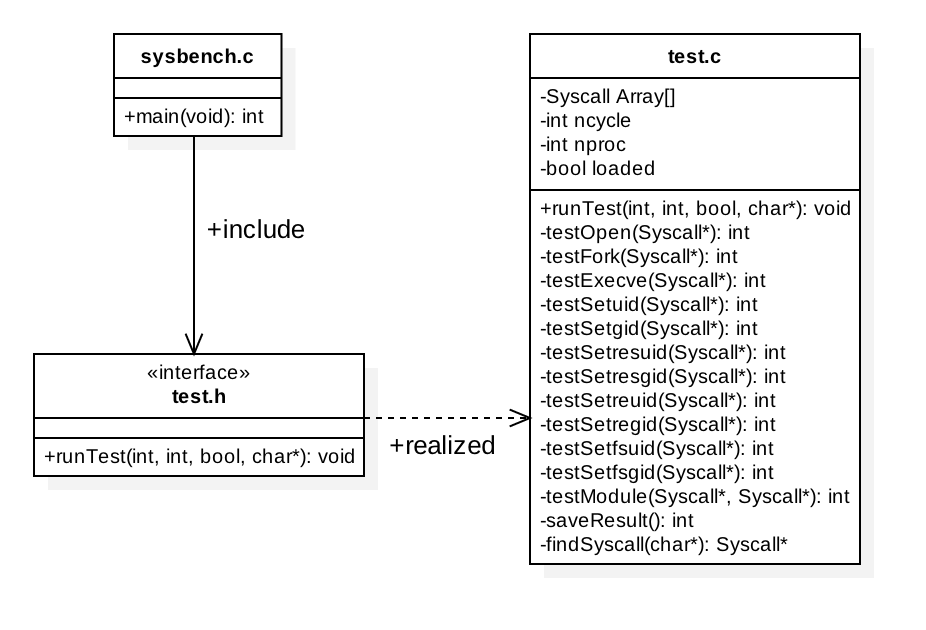
\includegraphics[scale=0.3]{Figures/Architecture}
\caption[Architettura del software SysBench]{Architettura del software SysBench.}
\label{fig:Architecture}
\end{figure}

La \autoref{fig:Architecture} mostra la struttura dei file del progetto e la loro interazione. Il \emph{main} è contenuto nel file \emph{sysbench.c}, in cui avviene il setup del programma che comprende la pulizia del prompt dei comandi, al fine di avere la finestra interamente dedicata a SysBench, e la verifica della presenza o meno di LKRG, la quale viene riportata assieme ai risultati nel file di output. Inoltre vengono letti i parametri passati da riga di comando, ovvero il numero di volte \emph{ncycle} che la singola system call verrà testata ed il nome del file \emph{filename} di output in cui vengono salvati i risultati. È importante prestare attenzione ad i parametri inseriti dall'utente, in quanto un malintenzionato potrebbe inserire codice malevolo per apportare modifiche dannose, dato che vengono richiamate funzionalità potenzialmente pericolose come la \emph{setuid()}. In merito a ciò, si è inserito il controllo di tale parametri al file di verificare la loro integrità.

Il file \emph{test.c} è un grosso ed unico sorgente nel quale vengono definite internamente tutte le funzioni utilizzate nel test; infatti, \emph{runTest()} che è l'unica funzione d'interfaccia è composta da un ciclo all'interno del quale vengono eseguite in serie tutte le valutazioni delle varie system call. Per scelta progettuale, si è deciso di creare la struttura \emph{Syscall} che rappresenta le varie chiamate di sistema da eseguire. È composta da:

\begin{itemize}
\item il nome in formato human-readable della funzione;
\item il puntatore alla funzione da eseguire, per fare si che ognuna di esse esegua il test opportuno (esempio: alla Syscall che testa la \emph{open()} verrà assegnato il test \emph{testOpen()} durante la creazione);
\item il tempo di esecuzione del test misurato in doppia precisione.
\end{itemize}

Durante la fase di progettazione del sistema si è prestata maggiore attenzione alla scalabilità, ovvero la possibilità di aggiungere/rimuovere funzionalità in maniera semplice ed efficace in base alle proprie esigenze. Grazie alla struttura del programma, è possibile aggiungere un ulteriore test di un'altra system call in maniera facile ed immediata: è sufficiente dichiarare una nuova Syscall all'interno dell'array in fase di inizializzazione, implementare la propria funzione \emph{testX()} ed assegnarla correttamente. Il sistema si preoccupa di soddisfare tutte le Syscall presenti, salvando il risultato di ognuna di esse independentemente dal numero.

Per risparmiare tempo, si è deciso di effettuare contemporaneamente sia il test di caricamento modulo sia quello di rimozione, in quanto non avrebbe senso scorporarli per il semplice motivo che il programma se deve effettuare l'inserimento di un modulo X volte, dovrà effettuare la sua rimozione altrettante volte al fine di non ricevere errore dalla funzione \emph{insert\_module()}, la quale fallisce se il target è già caricato nel kernel. Per questo è stata creata una funzione di utility \emph{findSyscall()}, la quale serve per ottenere il puntatore alla Syscall opposta a quella che si sta eseguendo (esempio: si sta testando la \emph{insert\_module()}, si deve trovare il puntatore alla \emph{delete\_module()} e viceversa), in maniera tale da salvare direttamente il risultato della funzione complementare all'interno della sua struttura.

Le funzionalità \emph{fork()} ed \emph{execve()} lavorano in maniera leggermente differente dalle altre; mentre solitamente la system call viene eseguita ncycle-volte come inserito dall'utente, queste due funzioni devono tenere conto del limite di processi istanziati dall'utente. È infatti possibile osservare tale limite leggendo il file \emph{/proc/self/limits} in cui vi è indicato il valore massimo oppure un'apposita struttura in C contenente tutti i limiti del sistema. Una volta letto questo valore, bisogna tenere conto anche dei processi al momento attivi nel sistema e la possibilità di lanciarne altri durante l'esecuzione di SysBench; per questo se il numero inserito dall'utente è troppo grande, fork() ed execve() potranno creare al massimo $ LIM / 2$, dove LIM è il valore letto in precedenza.

La system call \emph{execve()}, come riportato nella parte finale del capitolo precedente, sovrascrive tutto lo spazio dedicato al processo chiamante per eseguirne un altro e ciò potrebbe essere un problema dato che significherebbe la terminazione di SysBench non appena viene richiamata tale funzione. Come soluzione, si è scelto di far eseguire il comando ad un processo figlio, generato mediante la fork(), ottenendo così come tempo finale d'esecuzione la somma delle due chiamate a funzione. Quest'ultima feature è possibile grazie alla sincronizzazione tra i processo 'padre' ed i 'figli' utilizzando la funzione \emph{wait()}, grazie la quale il chiamante attende che tutti i suoi figli notifichino la loro terminazione, e solo in seguito procede con l'esecuzione del suo codice. Con questa soluzione non solo si riesce a misurare abbastanza accuratamente il tempo d'esecuzione dell'intera chiamata a funzione, ma il programma non genera dei processi definiti 'zombie', ossia processi creati e non terminati che rimangono in memoria in attesa di essere rimossi consumando inutilmente risorse

\section{Caso d'uso}

Essendo SysBench un software d'utility sviluppato per un utilizzo semplice e mirato, l'unico caso d'uso da commentare è il seguente mostrato in \autoref{fig:UseCase}.

\begin{figure}[!htbp]
\centering
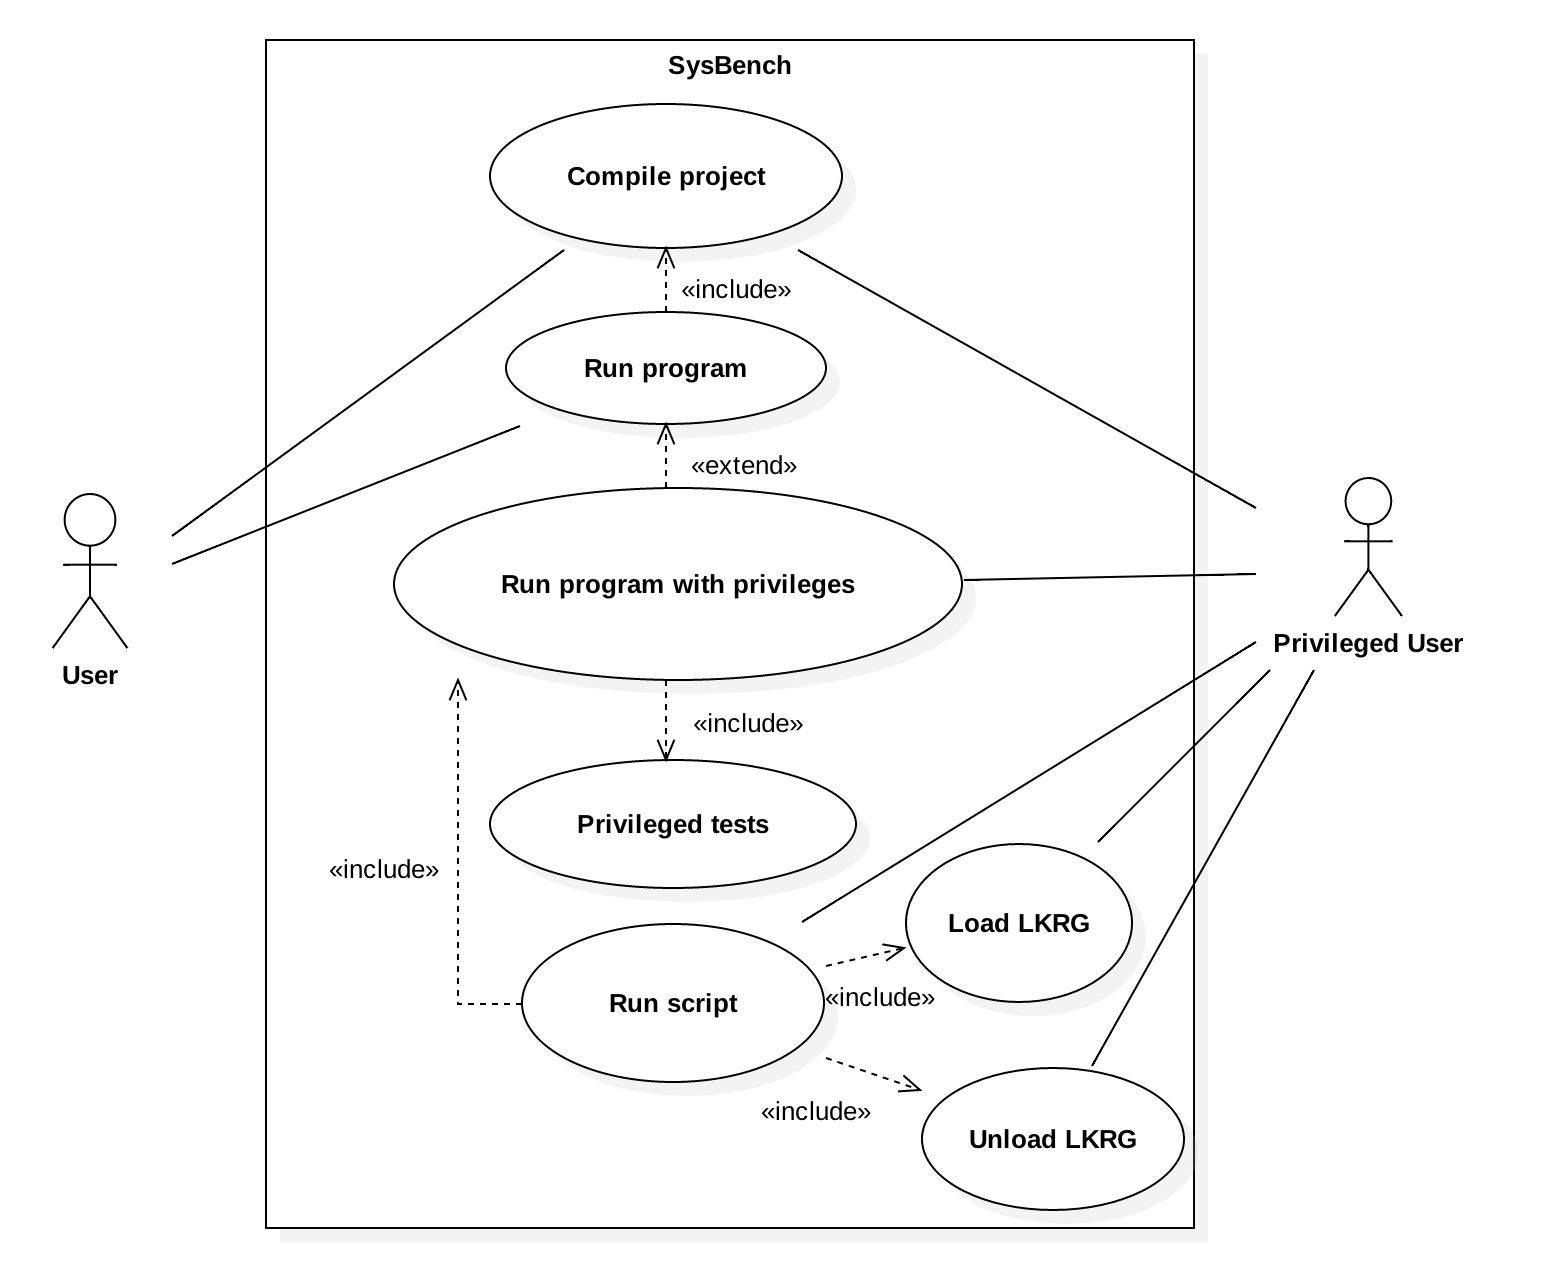
\includegraphics[scale=0.28]{Figures/UseCase}
\caption[Diagramma UML dei casi d'uso di SysBench]{Diagramma UML dei casi d'uso di SysBench.}
\label{fig:UseCase}
\end{figure}

Una volta compilato il progetto, è possibile procedere con due diverse modalità di esecuzione:

\begin{enumerate}
\item normal mode (\emph{./sysbench ncycle filename});
\item sudo mode (\emph{sudo ./sysbench ncycle filename})
\end{enumerate}
dove ncycle corrisponde al numero di volte che una singola chiamata di sistema viene invocata, mentre filename è il nome del file in cui verrano salvati i risultati all'interno della cartella \emph{output}, creata automaticamente nel caso non fosse già presente.

La differenza risiede nei test delle funzionalità di caricamento e rimozione modulo, ovvero \emph{testMoule()} (il quale richiama le system call \emph{insert\_module()} e \emph{delete\_module}); non è infatti possibile eseguire con successo questo test se non si hanno i privilegi di root, in quanto per scelta di sicurezza del sistema queste system call non possono modificare i moduli caricati nel kernel se eseguite da un normale utente (non a caso anche i comandi \emph{insmod} e \emph{rmmod} mostrati nel Capitolo I necessitano di tali privilegi).

Ad esclusione di questo test, tutti gli altri sono effettuati con successo in entrambe le modalità e falliscono solamente nel caso vi sia un errore interno al sistema. Nonostante l'utilizzo di sudo permetta di effettuare operazioni ritenute malevole da LKRG quindi non buone per il sistema, in questo progetto tutte le system call testate che prevedono un'alterazione di un parametro del processo si limitano ad impostare come valore dell'attributo quello corrente, in maniera tale da terminare con successo: ad esempio la \emph{setuid()}, utilizzata per cambiare l'identificatore dell'utente che ha lanciato il processo, imposta tale parametro al valore ritrovato in seguito alla system call opposta, ovvero \emph{getuid()}.

Vi è inoltre un'altra modalità d'esecuzione che prevede il caricamento e rimozione automatica di LKRG tra una valutazione di SysBench ed un'altra. Nel progetto è presente infatti uno script che richiede i privilegi di root per essere eseguito (per il motivo appena spiegato), grazie al quale viene eseguito il benchmark un numero di volte a piacere dall'utente. Si è infatti osservato che la differenza tra un'esecuzione singola di SysBench con ncycle=50 e 50 esecuzioni con ncycle=1 presentano risultati completamente differenti introdotti nel prossimo capitolo. Questa differenza è dovuta dalle ottimizzazioni e salvataggio in memoria cache delle funzioni invocate che permettono la loro immediata esecuzione, risparmiando al programma la loro ricerca nella tabella delle system call. È possibile eseguire lo script da riga di comando lanciando \\\emph{sudo ./script.sh ntimes ncycle path/to/p\_lkrg.ko} dove:

\begin{itemize}
\item ntimes è il numero di volte che verrà effettuato il benchmark;
\item ncycle è il numero di chiamate alle singole system call in ogni benchmark;
\item path/to/p\_lkrg.ko è il percorso del modulo compilato nel proprio sistema.
\end{itemize}

Nonostante i risultati ottenuti siano differenti, la possibilità di eseguire il programma con il parametro ncycle maggiore di 1 è stata volutamente lasciata, perchè i valori non solo sono interessanti per futuri sviluppi del progetto, ma anche per un'analisi delle ottimizzazioni di un calcolatore esterna a questo elaborato.